\documentclass[11pt]{article}

\usepackage[T1]{fontenc}
\usepackage{lmodern}
\usepackage[spanish,mexico,es-noshorthands,es-nosectiondot]{babel}
\spanishplainpercent
\usepackage[margin=2.5cm]{geometry}
\usepackage{booktabs}
\usepackage{graphicx}
\usepackage{float}
\usepackage[hidelinks]{hyperref}

\hypersetup{pdftitle={Lluvia y emergencias urbanas en Hermosillo}}

% Las cifras salen de notebooks/09-historia-lluvia-911.ipynb (historia y gráficas
% de docs/img/historia/) y de notebooks/08-exploracion-redefinicion.ipynb.

\begin{document}

\begin{center}
  {\LARGE Lluvia y emergencias urbanas en Hermosillo\par}
  \vspace{0.3em}
  {\large Qué puede esperar el 911 el día que llueve\par}
  \vspace{0.8em}
  Nombre del integrante 1 · correo@pendiente · LinkedIn o GitHub pendiente\\
  Nombre del integrante 2 · correo@pendiente · LinkedIn o GitHub pendiente\\
  Nombre del integrante 3 · correo@pendiente · LinkedIn o GitHub pendiente\\
  Nombre del integrante 4 · correo@pendiente · LinkedIn o GitHub pendiente\\[0.5em]
  Ingeniería de características, maestría en ciencia de datos. Corte: 15 de noviembre de 2026.
\end{center}

\section*{Resumen ejecutivo}

En Hermosillo llueve fuerte (10~mm o más en un día) unas seis veces al año, dos de cada tres veces de julio a septiembre, y esos días cambian la carga del 911. Un día seco de temporada recibe 1.7 llamadas de los tipos ligados al agua y al terreno; con 10 a 20~mm llegan 9 y con más de 20~mm entre 17 y 19, con días malos de más de 40. La carga sigue alta al día siguiente, son sobre todo árboles e inundaciones, y crece de madrugada.

Para el servicio esto se traduce en cuatro expectativas: usar el pronóstico de lluvia como aviso de demanda (ante 20~mm o más, unas diez veces un día seco, y alta también al día siguiente); reforzar los turnos de noche y madrugada después de una tormenta; coordinar antes de julio cuadrillas de retiro de árboles, bombeo y tapas de alcantarilla; y revisar 50 colonias que reinciden en tres años o más y reúnen 62\% de las llamadas ubicadas (San Benito, Balderrama, Sahuaro, Olivares y Centro, entre otras). Los baches y las fallas de agua potable no aumentan con la lluvia.

\begin{figure}[H]
  \centering
  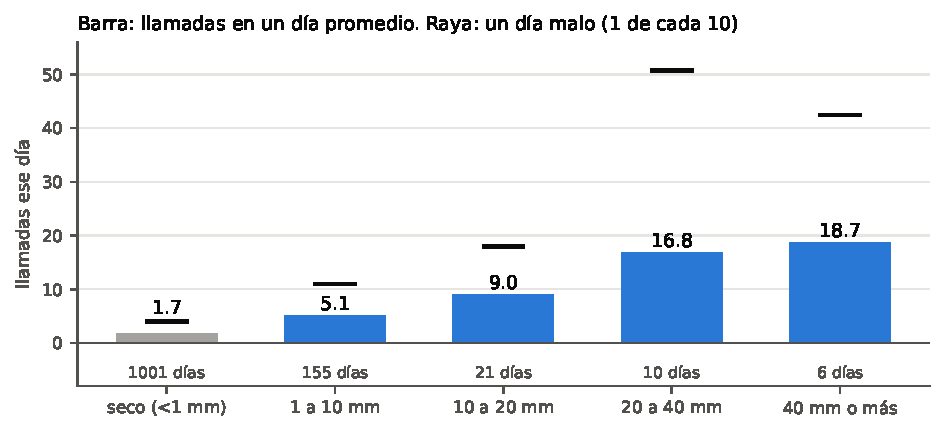
\includegraphics[width=0.6\textwidth]{../img/historia/2_intensidad.pdf}
  \caption{Llamadas al 911 en un día de junio a octubre según la lluvia de ese día, 2018 a 2025. Barra: promedio; raya: un día malo (solo 1 de cada 10 días de esa categoría lo supera). Fuentes: \cite{marcelinux2025,zippenfenig2023}.}
  \label{fig:intensidad}
\end{figure}

\begin{table}[H]
  \centering
  \caption{Cómo se arma la historia: qué aporta cada fuente y a cuál de las cuatro preguntas responde.}
  \label{tab:fuentes}
  \begin{tabular}{llc}
    \toprule
    Fuente & Qué aporta & Pregunta \\
    \midrule
    Llamadas al 911, 2018 a 2025 \cite{marcelinux2025} & La afectación: qué, cuándo y dónde & 1 a 3 \\
    Lluvia diaria, Open-Meteo \cite{zippenfenig2023} & Días tras lluvia frente a días secos & 1 a 4 \\
    Colonias y cauces, INEGI \cite{inegidcah,inegired} & Ubicación y cercanía a un cauce & 3 \\
    Bachómetro \cite{bachometro} & Contraste: calles dañadas & 4 \\
    Agua de Hermosillo \cite{aguah} & Contraste: emergencias del agua potable & 4 \\
    \bottomrule
  \end{tabular}
\end{table}

\paragraph{1. ¿Cuándo llama la ciudad al 911 por la lluvia?} Casi solo en verano. De julio a septiembre cae dos tercios de la lluvia del año, la del monzón \cite{adams1997}, y en esos mismos meses entra la mayor parte de las llamadas (figura~\ref{fig:calendario}); en los años secos, como 2023 y 2024, las llamadas por inundación casi desaparecen. Dentro de la temporada, lo que decide la carga es cuánto llueve ese día: cada escalón de lluvia sube el promedio de llamadas, hasta unas diez veces un día seco cuando pasan de 20~mm (figura~\ref{fig:intensidad}). Tras una tormenta fuerte, el día siguiente recibe tantas llamadas como el de la lluvia, unas cinco veces un día seco (figura~\ref{fig:fila}, izquierda).

\begin{figure}[!htb]
  \centering
  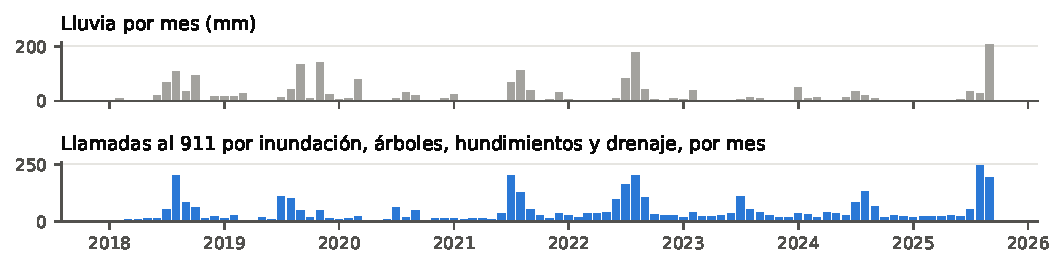
\includegraphics[width=0.68\textwidth]{../img/historia/1_calendario.pdf}
  \caption{Lluvia por mes y llamadas al 911 por mes, enero de 2018 a septiembre de 2025.}
  \label{fig:calendario}
\end{figure}

\paragraph{2. ¿Qué piden y a qué hora?} Saber cuándo llega la carga sirve si se sabe qué llega. Lo que más crece tras la lluvia son los árboles caídos y las inundaciones, seguidos de hundimientos, alcantarillas sin tapa y derrumbes (figura~\ref{fig:fila}, centro): trabajo de cuadrillas de poda, bombeo y obra, más que de ambulancias. Además, la carga cambia de horario: en días de lluvia el pico pasa de las 18:00 a las 21:00 y la madrugada recibe 12\% de las llamadas, cuatro veces lo de un día seco (figura~\ref{fig:fila}, derecha).

\begin{figure}[!htb]
  \centering
  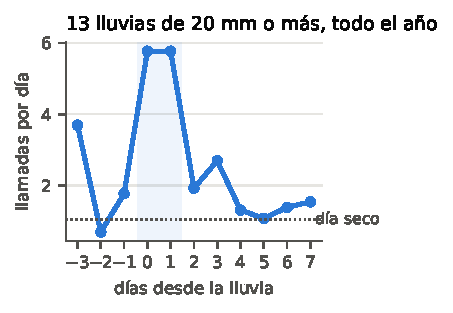
\includegraphics[width=0.32\textwidth]{../img/historia/3_dos_dias.pdf}\hfill
  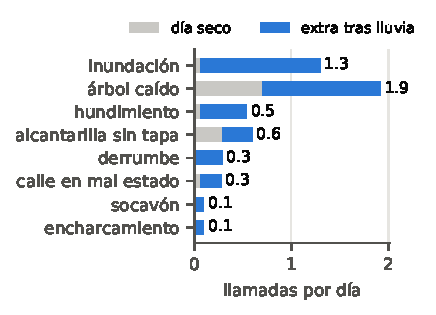
\includegraphics[width=0.34\textwidth]{../img/historia/4_tipos.pdf}\hfill
  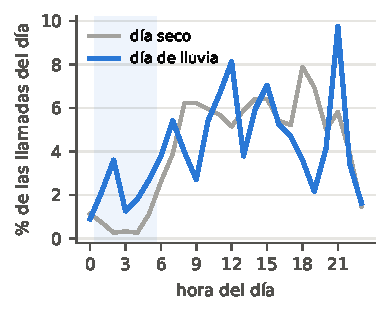
\includegraphics[width=0.32\textwidth]{../img/historia/5_horas.pdf}
  \caption{Izquierda: llamadas por día alrededor de una lluvia de 20~mm o más en cualquier mes (punteado: día seco del año). Centro: llamadas por día de cada tipo tras una lluvia de 10~mm o más (gris: día seco; azul: lo que agrega la lluvia). Derecha: porcentaje de las llamadas del día por hora.}
  \label{fig:fila}
\end{figure}

\paragraph{3. ¿Dónde?} Al cruzar el nombre de colonia que captura el 911 con el catálogo del INEGI se ubicaron dos de cada tres llamadas. Las colonias afectadas cambian de un año a otro, pero 50 se repiten en tres años o más y reúnen 62\% de las llamadas ubicadas (figura~\ref{fig:final}, izquierda). Son colonias grandes (área mediana siete veces la del conjunto), así que parte de su peso es su tamaño; aun así son la lista natural para revisar desagües, arbolado y tapas antes de julio.

\paragraph{4. ¿Pasa lo mismo con los otros servicios del agua?} Hasta aquí todo sale del 911. El proyecto empezó con otras dos fuentes: los reportes del Bachómetro y los avisos de Agua de Hermosillo. Si la lluvia también las moviera, el pronóstico serviría para esos servicios. No es así (figura~\ref{fig:final}, derecha): frente a días secos de la misma temporada, las llamadas por inundación suben 21.7 veces, pero los baches no cambian una vez que se compara dentro del mismo mes, y las emergencias de agua potable tampoco. En el texto de Agua de Hermosillo la lluvia sí aparece, como causa de apagones que detienen el bombeo, pero en episodios aislados. Por eso el tablero se centra en el 911.

\begin{figure}[!htb]
  \centering
  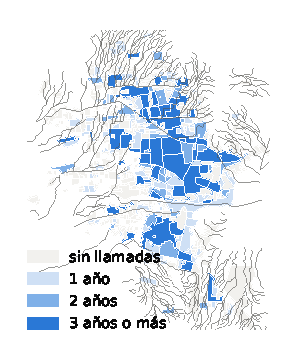
\includegraphics[width=0.25\textwidth]{../img/historia/6_colonias.pdf}\hspace{2em}
  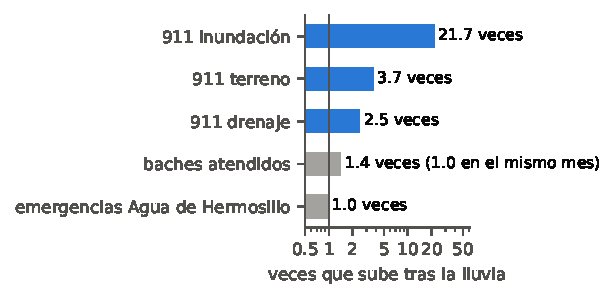
\includegraphics[width=0.44\textwidth]{../img/historia/7_no_lluvia.pdf}
  \caption{Izquierda: años con llamadas tras una lluvia de 10~mm o más por colonia, con los cauces en gris. Derecha: veces que sube cada serie tras una lluvia de 10~mm o más frente a días secos de junio a octubre (escala logarítmica).}
  \label{fig:final}
\end{figure}

\paragraph{Limitaciones.} La lluvia no viene de un pluviómetro en la ciudad sino de una estimación que promedia zonas de varios kilómetros y puede no registrar una tormenta local, así que las expectativas tienden a quedarse cortas. Una de cada tres llamadas no se ubicó en una colonia y no hay población por colonia. Detalle: notebooks 08 y 09.

\begin{thebibliography}{10}
\raggedright

\bibitem{adams1997}
Adams, D. K. y Comrie, A. C. (1997). The North American Monsoon. Bulletin of the American Meteorological Society, 78(10), 2197-2213. \url{https://doi.org/10.1175/1520-0477(1997)078<2197:TNAM>2.0.CO;2}

\bibitem{aguah}
Agua de Hermosillo. Publicaciones de la página oficial de Facebook, diciembre de 2020 a septiembre de 2026. Snapshot descrito en \texttt{data/SNAPSHOT.md}.

\bibitem{bachometro}
H. Ayuntamiento de Hermosillo. Bachómetro. \url{https://bachometro.hermosillo.gob.mx}

\bibitem{inegidcah}
INEGI (2025). Delimitación de colonias y otros asentamientos humanos (DCAH). \url{https://www.inegi.org.mx/programas/dcah/}

\bibitem{inegired}
INEGI. Red Hidrográfica escala 1:50 000, edición 2.0. \url{https://www.inegi.org.mx/temas/hidrografia/}

\bibitem{marcelinux2025}
Marcelinux (2025). Llamadas 911 por colonia, Hermosillo 2018-2025. Hugging Face, CC-BY-4.0. \texttt{huggingface.co/datasets/Marcelinux}

\bibitem{zippenfenig2023}
Zippenfenig, P. (2023). Open-Meteo.com Weather API. Zenodo. \url{https://doi.org/10.5281/zenodo.7970649}

\end{thebibliography}

\end{document}
